\section{Case Study and Gallery}
\label{sec:case-studies}

We demonstrate {\system} through a representative authoring case and five
additional examples spanning different chart families, coordinate
systems, data structures, and composition types (Fig.~\ref{fig:teaser}), which can be inspected in our online gallery
(\url{https://visbricks.github.io/}).

\textbf{Progressive construction.}
A scatterplot is first created to examine the joint distribution of two
dimensions, together with an area chart that aggregates the data along the
$x$ dimension to summarize the marginal distribution of points. An additional
nominal dimension describing the composition of each point is then introduced
by nesting a pie chart within the scatterplot points. Each nested instance
inherits the data context of its corresponding point.
The same dimension can subsequently be introduced into the configured area
chart. Because the current area block cannot accommodate the additional
dimension, {\system} exposes alternative adaptations, including switching to a
higher-capacity form in the same family, such as a stacked area or streamgraph,
or faceting the existing area chart by the new dimension. In this example, a
streamgraph is selected as the desired visual form. The resulting composite
visualization is shown in Fig.~\ref{fig:teaser}(a).

\textbf{Gallery examples.}
The remaining cases show how different chart units and composition operations
support a broader range of structures. (b) concatenates a sunburst and a
dendrogram in polar coordinates. (c) layers geographic point, link, and
heatmap units to form a geographic network view, and further nests stacked bar
charts within network nodes. In (d), pie charts are positioned according to a
scatterplot, graph links are layered over them, and stacked bar charts are
concatenated along the top and right margins to summarize the aggregated
composition of the pies. In (e), a chord diagram is combined with circular
stacked bar charts in polar coordinates. The bar chart is first faceted by
\texttt{node\_id}, producing repeated views in a new polar layout, and these
views are then concatenated with the chord by aligning them to the
corresponding node angles. Finally, (f) uses a dendrogram as the parent
structure and nests a composite unit consisting of a radial stacked bar chart
and an area chart within its nodes. Together, these examples demonstrate how
layering, concatenation, nesting, and faceting can be applied to different
units while retaining the same block-based authoring logic.


\section{User Study}

We conducted a user study consisting of two complementary parts: a comparative
study and an exploratory study. The comparative study examined the authoring
workflow of {\system} against existing tools, while the exploratory study
investigated whether its authoring logic could be transferred across different
visualization designs. 
The study was approved through our lab's internal research review process.

\textbf{Participants.}
We recruited 12 participants (P1--P12; 7 male, 5 female) with experience in
authoring composite visualizations. Their backgrounds included dashboard
creation, visual analytics system design, and visualization research or
development. They were familiar with visualization tools or grammars such as
D3.js~\cite{D3} and Vega-Lite~\cite{VegaLite}, as well as
fundamental visualization concepts such as visual encoding channels and the
binding of data attributes to these channels. In the comparative study, we
compared {\system}, Tableau~\cite{Tableau}, and Data Illustrator~\cite{DataIllustrator}
(Hereafter, we refer to Data Illustrator as DI.); none of the participants had prior hands-on
experience with Tableau or DI. All participants completed both parts of the
study.

\subsection{Comparative User Study}
\label{sec:comparative-study}

We conducted a comparative user study to examine how {\system}, DI, and
Tableau support the implementation of a predefined visualization design. The
study focused on differences in their authoring workflows for constructing and
organizing the specified visual structure.

\subsubsection{Study Design}

We designed the study and training protocol to support a controlled comparison
across the three systems while ensuring that participants had the basic
operational knowledge required for each condition.

\textbf{Task.}
Participants were asked to reproduce the visualization shown in
\autoref{fig:teaser}(a) using each system, with the same input dataset and
target visualization across all conditions. They were expected to reproduce
the main visual elements, data encodings, and overall structure, while
annotations and minor stylistic details were not required.

\textbf{Order.}
The study followed a within-subject design, with each participant completing
the task using all three systems. We
used complete counterbalancing: the 12 participants were evenly assigned to
the six possible system orders, with two participants following each order.

\textbf{Preliminary testing and training.}
We conducted preliminary walkthroughs with the authors and informal pilot
sessions with two users who did not participate in the main study. These
sessions identified the task-relevant features to introduce and informed the
training duration: approximately 6 minutes for both {\system} and Tableau and
12 minutes for DI, which required more time to cover the relevant operations.
The durations were intended to ensure basic operational readiness rather than
equal exposure. Training covered only task-relevant features and did not
demonstrate how to reproduce the target visualization.

\subsubsection{Procedure}

Each study session consisted of an orientation, three system-specific task
sessions, and a concluding interview.

\textbf{Orientation.}
The facilitator first introduced the overall study procedure. Participants
then received a 10-minute overview of the input dataset and target
visualization, including the relationships between data fields and visual
elements. This overview was system-independent and intended to ensure a shared
understanding of the task.

\textbf{Task sessions.}
For each system, participants first completed the corresponding training and
practice activities. They then independently reproduced the target
visualization within a 20-minute time limit. Task completion time was measured
from the beginning of the reproduction task and excluded training and
practice.
During the task, facilitator assistance was provided only for operational
difficulties. We recorded an assistance instance in either of two situations:
(1) a participant explicitly requested help because they did not know how to
proceed, or (2) the participant performed a clearly incorrect operation that
prevented correct task progression and required facilitator correction. Both
types were treated as operational assistance because they indicated that the
participant could not proceed independently at that point. Assistance was
limited to clarifying how to use system features or identifying the incorrect
operation; the facilitator did not recommend authoring strategies or make
design decisions on behalf of the participant. The same assistance protocol
was applied across all three systems.
After each task session, participants completed an 11-item questionnaire using
7-point Likert scales, which typically took 2--3 minutes.

\textbf{Concluding interview.}
After completing all three task sessions, participants took part in a
semi-structured interview lasting approximately 7 minutes. They were asked to
explain their questionnaire ratings, compare their authoring strategies and
workflows across the three systems, and discuss the advantages and difficulties
they encountered.

\textbf{Measures and analysis.}
We collected questionnaire ratings, task completion time, and the number of
assistance instances. The post-task questionnaire was organized around four
dimensions of authoring experience: learnability (2 items), compositional
usability (3 items), cognitive ease (3 items), and interaction intuitiveness
(3 items). All 11 items used 7-point Likert scales, with higher scores
consistently indicating a more favorable experience. For each dimension, we
averaged the corresponding item ratings within each participant and report
participant-level means and standard deviations.
Task completion time was used to characterize authoring efficiency, while the
number of assistance instances was used as an indicator of operational
independence after training. Requested and corrective assistance followed the
same counting rule and were aggregated for the primary analysis. We also
collected task observations and qualitative feedback from the concluding
interview to contextualize the quantitative measures. Full questionnaire
wording is provided in the supplementary material.


\subsubsection{Results}

We organize the comparative results around four aspects of the authoring
experience: learnability and operational independence, compositional
usability, interaction quality, and authoring efficiency. Questionnaire
ratings are summarized in Fig.~\ref{fig:comparative-ratings}, while task
completion time and assistance requests are reported in
Fig.~\ref{fig:comp_ef}.

\begin{figure}[t]
\centering
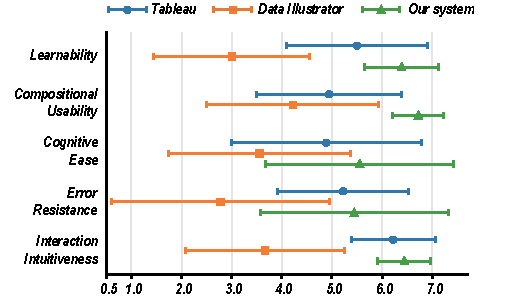
\includegraphics[width=\columnwidth]{figs/comp.pdf}
\caption{Participant ratings in the comparative study across learnability,
compositional usability, cognitive ease, error resistance, and interaction
intuitiveness for {\system}, Tableau, and Data Illustrator.}
\label{fig:comparative-ratings}

\end{figure}

\textbf{Learnability and operational independence.}
{\system} received the highest learnability ratings, while both {\system} and
Tableau required relatively little assistance. Participants generally found
Tableau's data-to-channel mapping easy to learn after training and noted that
assigning fields to the same channels produced relatively consistent effects.
With {\system}, participants particularly valued the explicit chart
thumbnails: once the intended visual form was identified, they could directly
select a corresponding block.
DI caused more difficulty at finer structural levels. Eight
participants made errors when selecting the level at which an encoding should
be applied, such as selecting an entire pie rather than its segments or an
individual element rather than its classified group. P5 described this process
as closer to ``thinking in code,'' requiring them to reason about intermediate
data filtering and hierarchical relationships. Although P5 considered this
model rigorous, they felt that it reduced intuitiveness. These observations
suggest that explicit visual forms in {\system} and stable channel semantics in
Tableau reduced operational knowledge participants needed to retain.



\textbf{Compositional usability.}
The largest rating difference between {\system} and the baseline systems
occurred in compositional usability
(Fig.~\ref{fig:comparative-ratings}). Participants consistently found the
composite structure in {\system} easier to interpret. For the nested portion of
the target visualization, most participants naturally described the design as
placing a pie chart inside points of a scatterplot, closely matching
{\system}'s block-and-composition model.
P8 contrasted this with Tableau and DI, which they described as
more top-down. DI progressively subdivides graphical structure
before binding data, whereas Tableau first partitions data and reflects those
partitions in the resulting view. P8 felt that both approaches were less
directly aligned with how they conceptually decomposed the visualization.
These responses suggest that explicit blocks and composition relationships
helped participants reason about composite structures in terms of recognizable
visual units.

\textbf{Interaction quality.}
{\system} received the highest ratings for cognitive ease, error resistance,
and interaction intuitiveness, while DI received the lowest
ratings on all three dimensions
(Fig.~\ref{fig:comparative-ratings}). Participants generally considered the
spatial interactions in {\system} intuitive and resistant to error. In
contrast, DI was repeatedly described as requiring more learning
and being more susceptible to selection errors, consistent with the
structural-level mistakes observed during the task.
P6 nevertheless identified a limitation of {\system}: nesting at the element
or group level was conceptually less straightforward than chart-level
composition operations such as concatenation and layering. This distinction
introduced additional reasoning when moving between chart-level and
element-level composition. Overall, the perceived advantage of {\system} was
therefore most pronounced in composition rather than uniformly across all
interaction measures.

\begin{figure}[t]
\centering
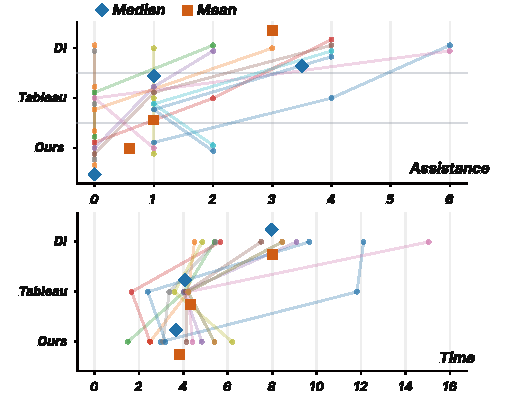
\includegraphics[width=\columnwidth]{figs/comp_ef.pdf}
\caption{Objective performance in the comparative study, showing task
completion time and the number of assistance requests for {\system}, Tableau,
and Data Illustrator for each participants.}
\label{fig:comp_ef}

\end{figure}

\textbf{Authoring efficiency.}
Participants completed the target fastest with {\system}, followed by Tableau
and DI (Fig.~\ref{fig:comp_ef}). Completion times differed
significantly across systems (Friedman $\chi^2(2)=9.77$, $p=.008$). Pairwise
comparisons showed that {\system} was faster than DI
(Holm-adjusted $p=.023$), while the difference between {\system} and Tableau
was not significant ($p=.910$).
P6 attributed the relative efficiency of both {\system} and Tableau to their
reliance on recognizable mark types and channel binding, which avoided much of
the fine-grained structural decomposition required in DI.
However, P6 also noted that DI's lower-level control could be
useful in more open-ended scenarios where exploring the design itself is more
important than implementing a predetermined design. Together with the
assistance results, these findings suggest that {\system} supported efficient
implementation of the prescribed composite visualization.


\subsection{Exploratory User Study}

This study aims to examine whether participants could transfer the authoring logic learned previously to unfamiliar visualization structures.


\subsubsection{Study Setting and Procedure}

The study followed the comparative study, with participants receiving a brief
introduction to key structural differences before each new task.

\textbf{Tasks.}
Participants reproduced three target visualizations using
{\system}, as shown in \autoref{fig:teaser}(b, c, f). Compared with the
target in the comparative study, these cases introduced polar and
geographic coordinate systems, hierarchical and network structures, and
layering operations not encountered. The tasks were
selected to examine whether participants could reuse learned
concepts and apply the same authoring logic across these varied visualization
structures.

\textbf{Procedure.}
The exploratory study lasted approximately 30 minutes. Before each task, the
facilitator briefly introduced the target visualization, including its input
data, channel encodings, and any chart types, coordinate systems, or operations
not encountered in the comparative study. These introductions did not
demonstrate the construction process or prescribe a sequence of operations.
Participants then reproduced each target using {\system} and determined the
construction process themselves. When participants were unable to proceed, the
facilitator could clarify the input data or the meaning of a system operation
but did not recommend a construction strategy or make authoring decisions on
their behalf. After completing all three tasks, participants filled out a
7-point Likert-scale questionnaire and provided open-ended feedback.

\textbf{Measures and analysis.}
The exploratory questionnaire was organized around five dimensions aligned
with our evaluation goals: block and family alignment (3 items), interaction
consistency (4 items), transferability (5 items), outcome predictability
(3 items), and expressive flexibility (5 items). All 20 items used the same
7-point Likert scale and were analyzed following the same procedure as in the
comparative study. We also collected task observations and open-ended
feedback to contextualize the questionnaire results. Full questionnaire
wording is provided in the supplementary material.



\subsubsection{Results}

All participants completed the exploratory tasks. We examined whether the
authoring logic learned in the comparative study remained applicable across
different chart types, coordinate systems, and composition structures.
Questionnaire ratings are summarized in
Fig.~\ref{fig:exploratory-ratings}, together with participants' qualitative
feedback.

\begin{figure}[t]
\centering

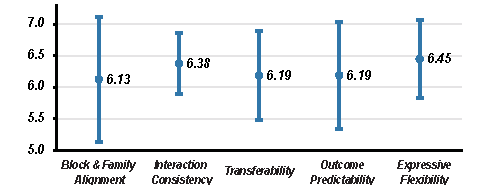
\includegraphics[width=\columnwidth]{figs/explo.pdf}

\caption{Participant ratings in the exploratory study.}
\label{fig:exploratory-ratings}

\end{figure}

\textbf{Alignment with blocks and families.}
Participants generally found that the provided blocks matched the visual units
into which they would decompose the target visualizations and that required
charts could usually be found in the families they expected. Block and family
alignment received positive ratings overall ($M=6.13$, $SD=0.99$).
P5 particularly valued the family thumbnails, noting that they made related
visual forms visible when changing dimensionality and helped reveal
alternatives that they might not otherwise know were available. Family
organization was not always interpreted uniformly, however. P9 expected to
find a sunburst chart in an arc-related family, whereas {\system} placed it in
the tree family according to its underlying data structure. This mismatch
suggests that perceptual family organization is not universal and that the
classification derived from the expert study may not fully reflect every
author's expectations.

\textbf{Consistency and transferability.}
Participants rated both interaction consistency and transferability highly.
The interaction logic remained consistent across the exploratory cases
($M=6.38$, $SD=0.49$), while participants also reported that operations
learned from the comparative task could be reused for unfamiliar designs
($M=6.19$, $SD=0.70$).
P7 summarized the workflow as unchanged: authors still configured individual
units and then composed them, although new chart types could require learning
their available encoding channels. Once the units were configured, the same
composition operations could be reused.
Polar concatenation was the main source of confusion. Participants sometimes
had difficulty distinguishing whether the angular or radial dimension was
being shared. After seeing the resulting compositions, however, they generally
found the behavior understandable. P10 noted that the drop zones themselves
provided useful graphical cues, making planar and ring-like concatenation
easier to understand visually than through the corresponding $\theta$- and
$r$-axis terminology.

\textbf{Outcome predictability.}
Participants rated outcome predictability positively across the exploratory
cases ($M=6.19$, $SD=0.84$). Layering and nesting were generally considered
highly predictable, whereas polar concatenation produced more hesitation and
occasionally required assistance.
P1 described a progression in predictability across the compared authoring
approaches. In DI, some encoding operations produced outcomes
they did not anticipate. In Tableau, the general role of a mark or channel
could be anticipated, but the final visual form often became clear only after
additional fields were assigned. In contrast, P1 found {\system}'s explicit
chart thumbnails useful because the resulting visual form was visible before
data configuration. P10 similarly reported difficulty predicting the effects
of some position-related encodings in DI, such as $x$, $y$, and
size properties, and noted that some operations remained difficult to
understand even after receiving assistance.
These responses suggest that explicit blocks and consistent composition
semantics helped make structural consequences visible in advance, while
predictability decreased when participants had to reason about unfamiliar
coordinate or low-level encoding semantics.

\textbf{Expressive flexibility.}
Expressive flexibility received the highest aggregate rating among the
exploratory dimensions ($M=6.45$, $SD=0.61$). Participants generally felt that
the expanded set of chart families, coordinate systems, and composition
structures broadened the range of visualizations they could construct without
changing the overall authoring logic.
P6 emphasized that the alternatives provided within chart families offered
both additional design options and inspiration: the composition operations
remained unchanged, while variation in the constituent units increased the
expressive range of the resulting compositions. P3 similarly noted that the
introduction of different coordinate systems together with tree and network
blocks substantially broadened both the visual forms and data relationships
that could be represented. These comments suggest that much of the perceived
increase in expressiveness came from expanding the vocabulary of composable
units rather than introducing separate authoring workflows.
